\subsection{Generación de señalamiento paso a paso}

\lipsum[1]

\begin{figure}[H]
	\centering
	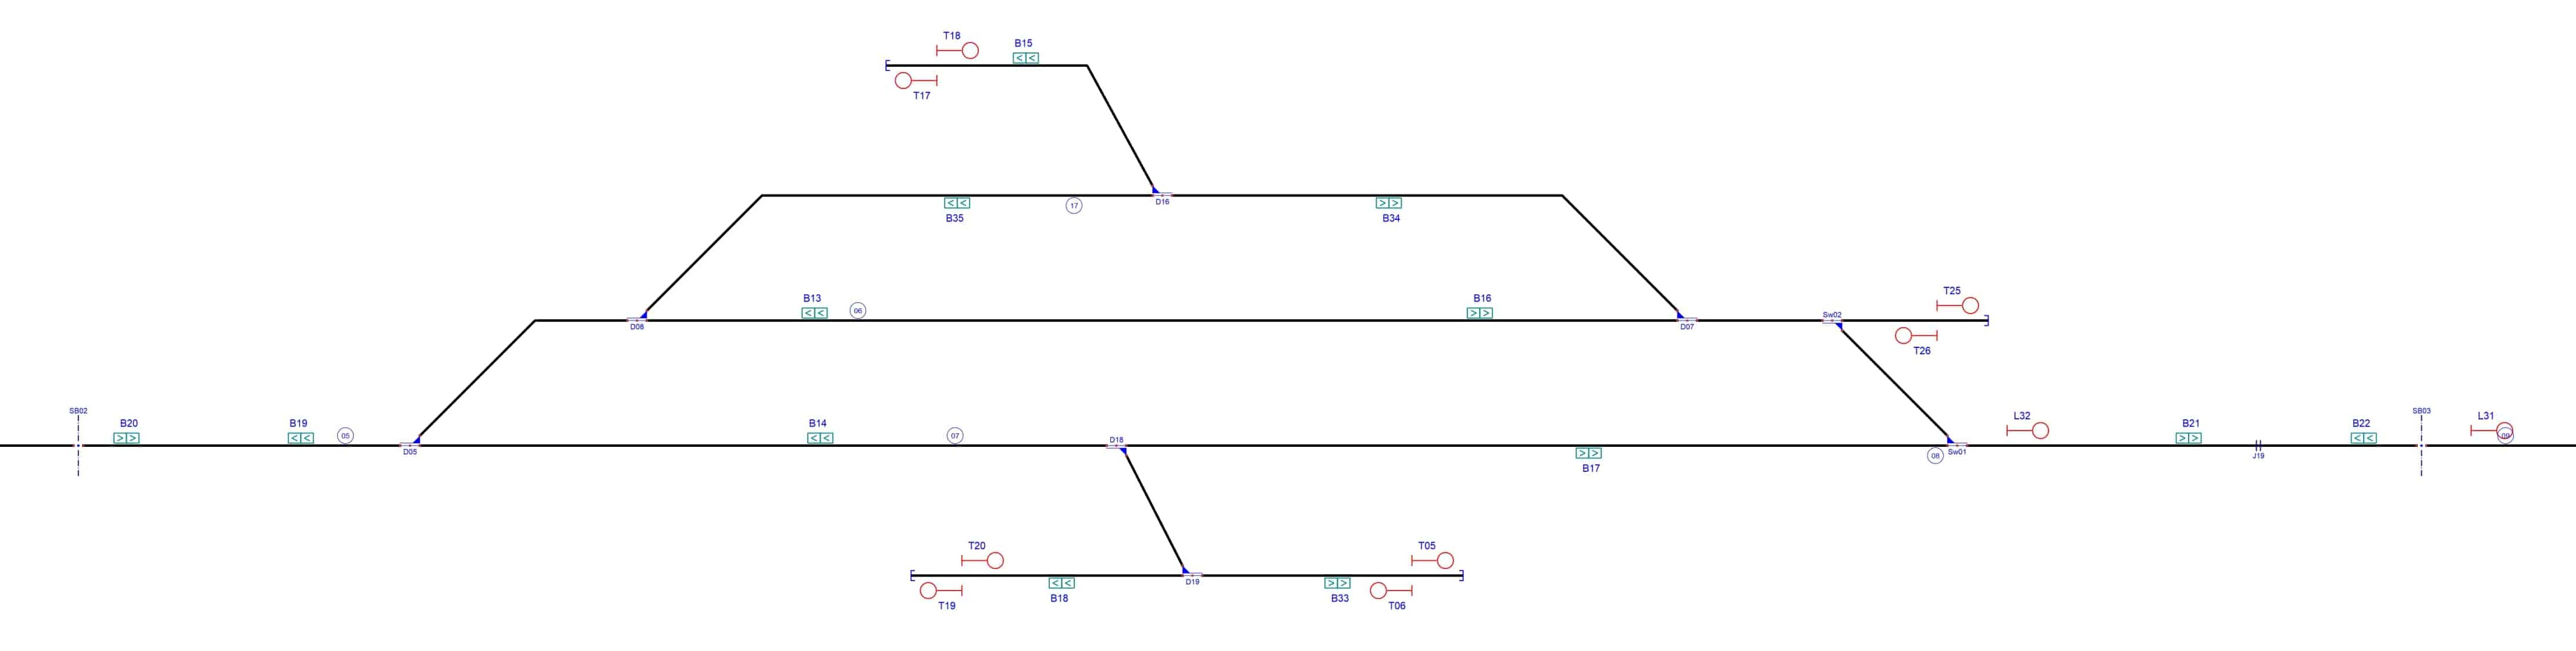
\includegraphics[width=1\textwidth]{resultados-obtenidos/ejemplo4/images/4_step1.png}
	\centering\caption{Señalamiento generado por el RNA para proteger el fín de vía.}
	%\label{fig:LC_P2}
\end{figure}

\lipsum[1]

\begin{figure}[H]
	\centering
	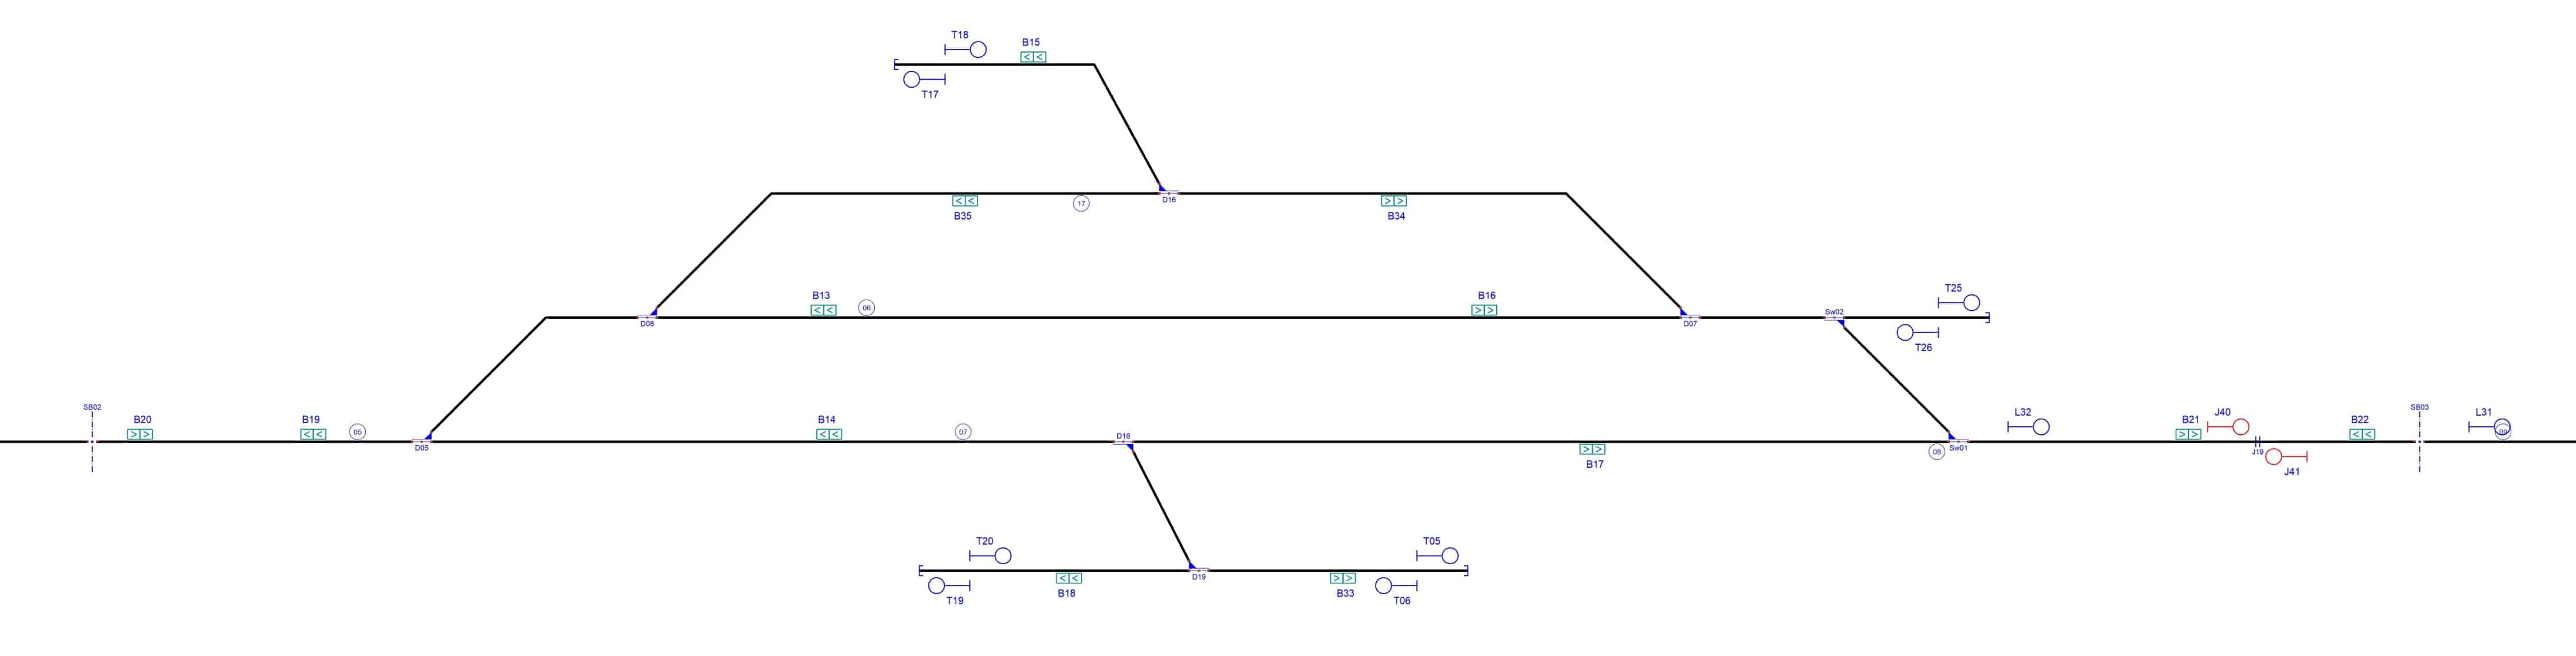
\includegraphics[width=1\textwidth]{resultados-obtenidos/ejemplo4/images/4_step2.png}
	\centering\caption{Señalamiento generado por el RNA para proteger las junturas.}
	%\label{fig:LC_P2}
\end{figure}

\lipsum[1]

\begin{figure}[H]
	\centering
	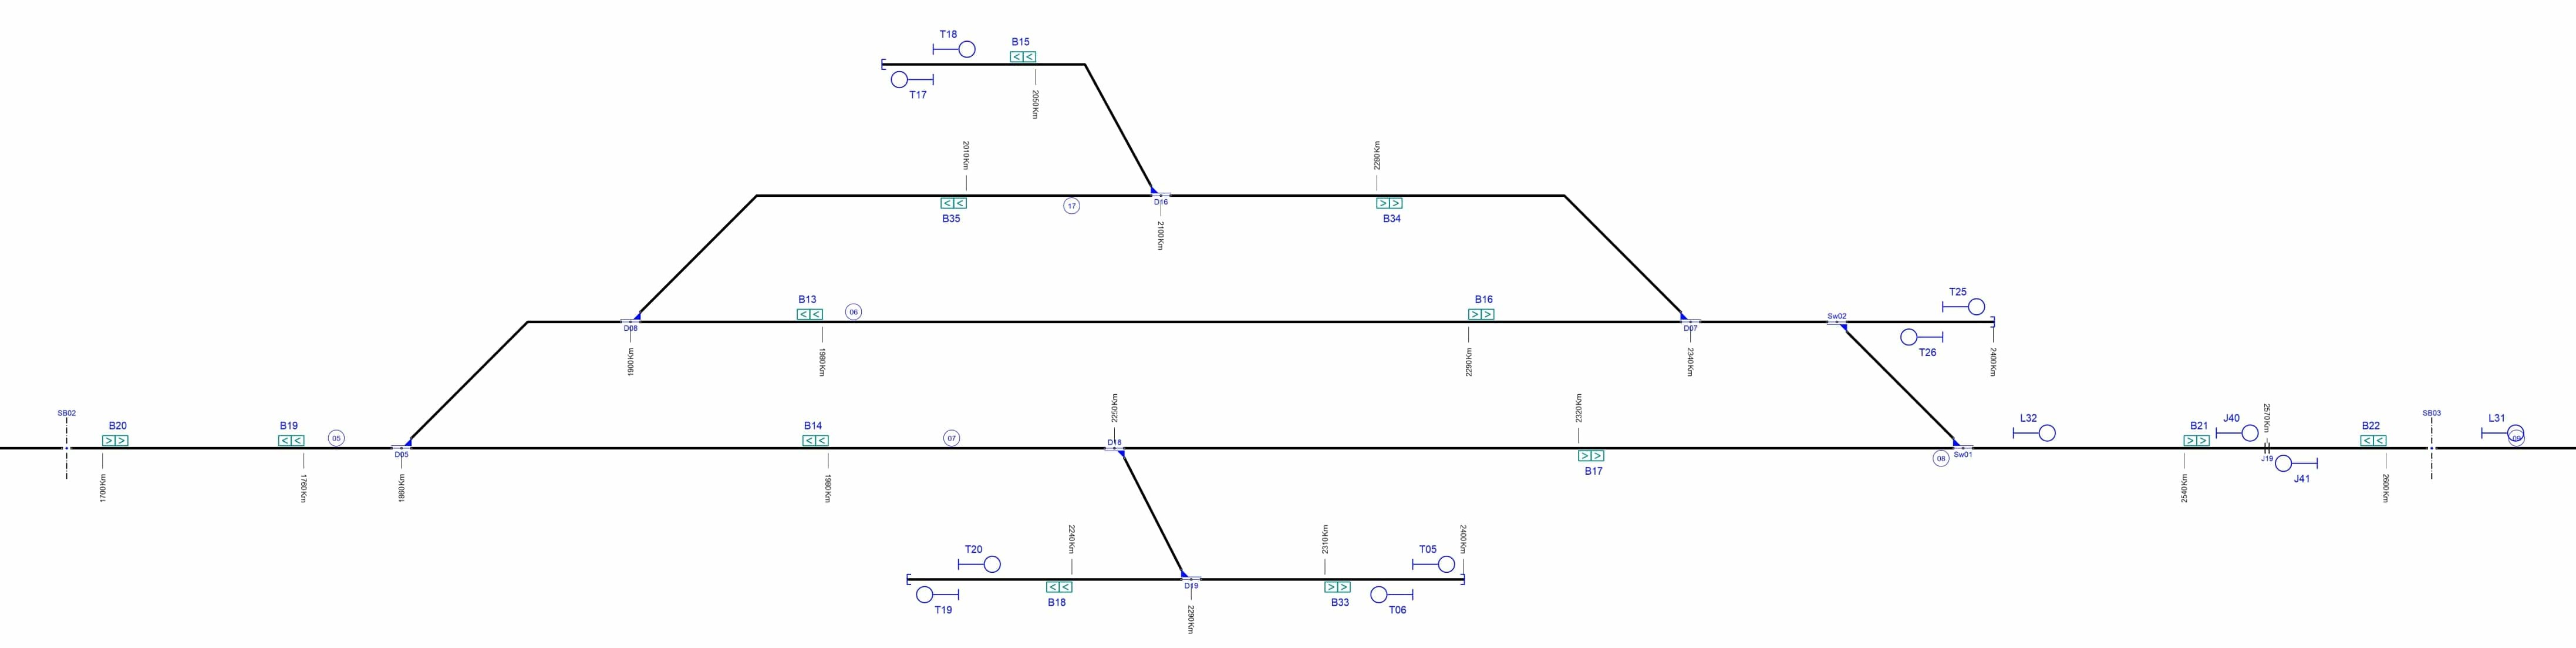
\includegraphics[width=1\textwidth]{resultados-obtenidos/ejemplo4/images/4_step3.png}
	\centering\caption{Señalamiento generado por el RNA para proteger plataformas y cruces de vía.}
	%\label{fig:LC_P2}
\end{figure}

\lipsum[1]

 \begin{figure}[H]
	\centering
	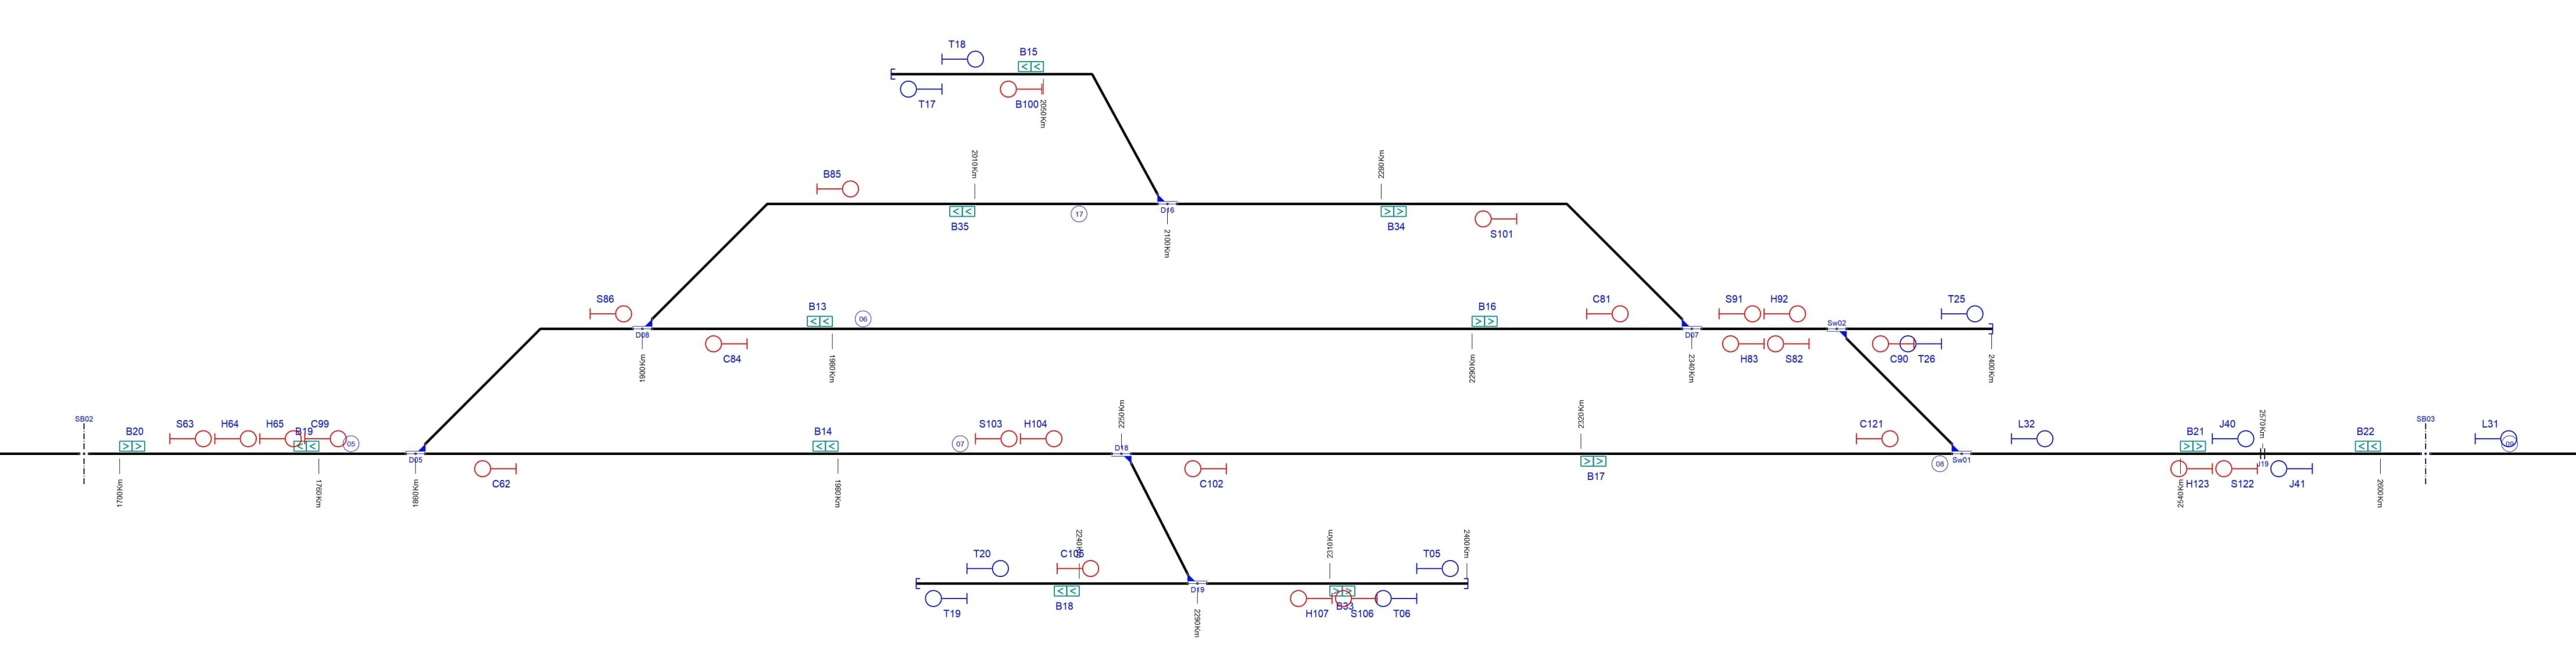
\includegraphics[width=1\textwidth]{resultados-obtenidos/ejemplo4/images/4_step4.png}
	\centering\caption{Señalamiento generado por el RNA para proteger las máquinas de cambios.}
	%\label{fig:LC_P2}
\end{figure}

\lipsum[1]

 \begin{figure}[H]
	\centering
	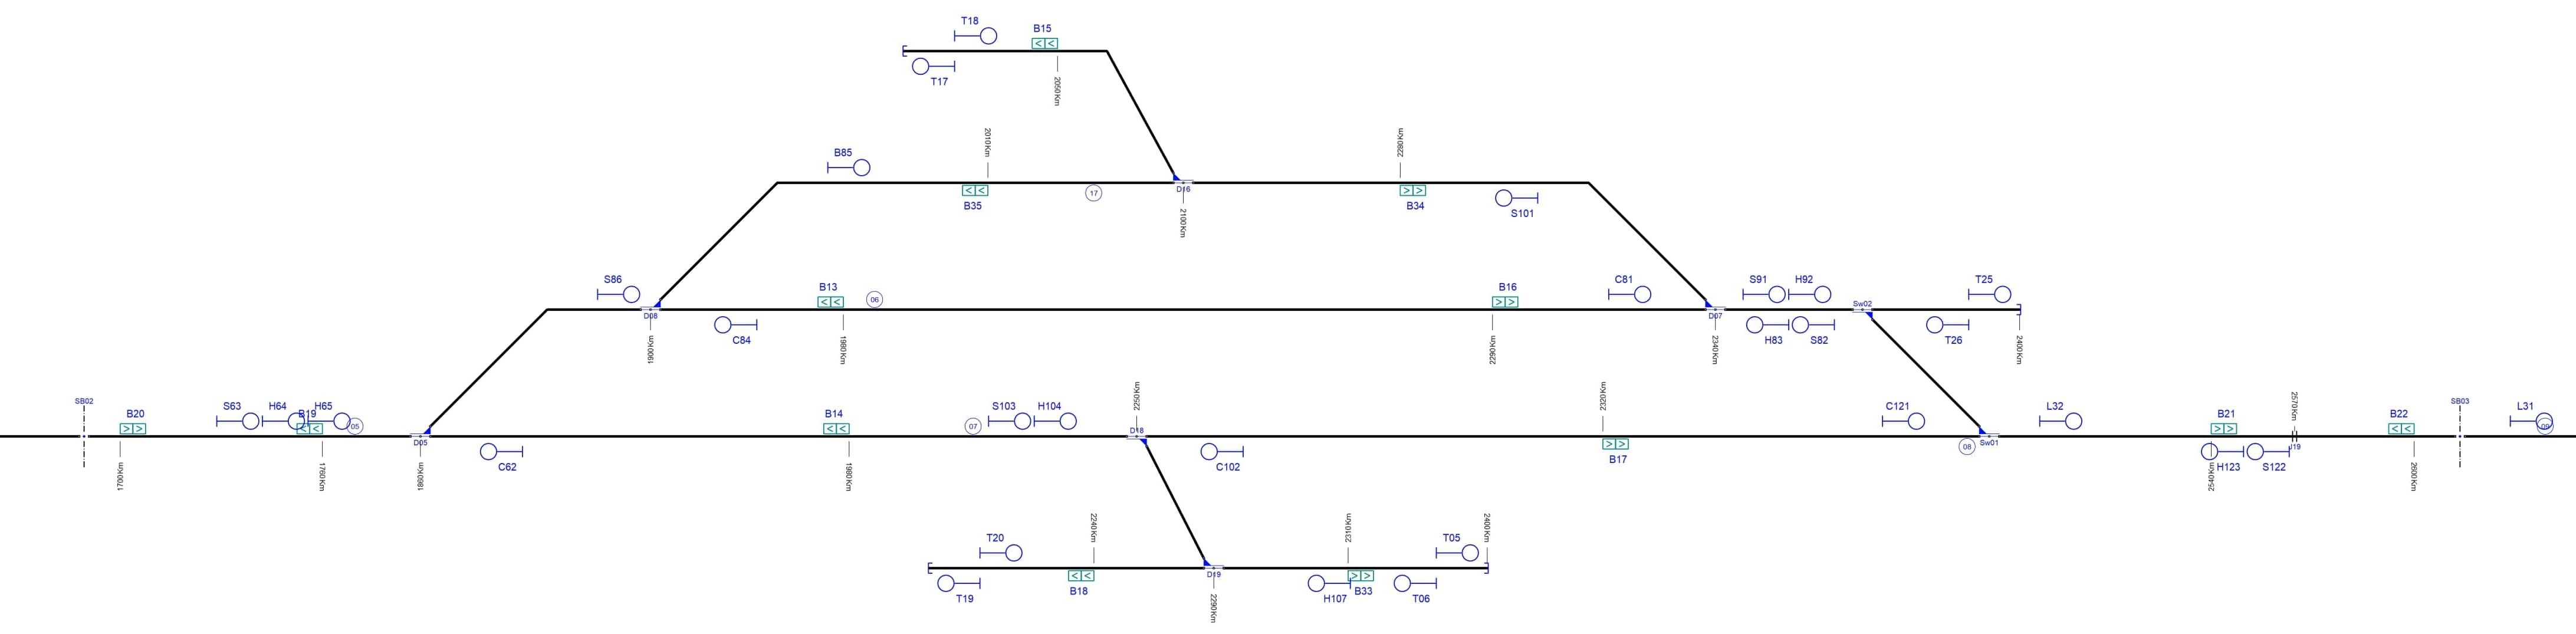
\includegraphics[width=1\textwidth]{resultados-obtenidos/ejemplo4/images/4_RNA.png}
	\centering\caption{Señalamiento generado y simplificado por el RNA.}
	%\label{fig:LC_P2}
\end{figure}

\lipsum[1]